\documentclass[11pt]{article}
\usepackage[margin=1in]{geometry}
\usepackage{amsmath,amssymb}
\usepackage{graphicx}
\usepackage{booktabs}
\usepackage[hidelinks]{hyperref}
\usepackage[numbers,sort&compress]{natbib}

% DRAFT drafted by Claude (AI) for the researcher to review and edit.
% Results are placeholders until the pre-registered analysis has run.

\title{Where in the brain is ``zoning out''? Pre-stimulus signatures of latent engagement states across the mouse brain, with cross-laboratory replication}
\author{[AUTHORS --- TBD]}
\date{DRAFT --- \today}

\newcommand{\todo}[1]{\textbf{[#1]}}

\begin{document}
\maketitle

\begin{abstract}
\todo{Write after results. One sentence each: problem; approach (GLM-HMM engagement states, IBL Brain-Wide Map, pre-stimulus decoding with block-prior and movement controls, session-permutation nulls, pre-registration); main result for H1--H3; replication in Steinmetz et al.\ 2019; implication.}
\end{abstract}

% =====================================================================
\section{Introduction}

Animals performing a task are not equally engaged from one trial to the next. In some stretches of trials, their choices closely follow the sensory evidence; in others, they guess, repeat a previous response, or lean towards one side regardless of what is shown. In mice trained on a visual decision task, these fluctuations are not random noise around one fixed strategy. A hidden Markov model whose states each have their own generalised linear model of choice (a GLM-HMM) shows that mice switch between a small number of discrete strategies. One is an ``engaged'' state with high stimulus sensitivity, and the others are ``disengaged'' or biased states. Each state typically lasts for tens of trials \citep{ashwood2022}. Related latent-state models have revealed internal states that shape behaviour in other species and tasks \citep{calhoun2019}. The factors that govern switching between states in the International Brain Laboratory (IBL) task, which has a changing block structure, are now being characterised from behaviour \citep{mohammadi2025}.

Because these states are inferred from choices alone, a central question is what they correspond to in the brain. One possibility is that engagement is set by a specific circuit, such as arousal-related midbrain structures or frontal and motor areas that prepare actions. Another is that it reflects a brain-wide change in state. A third is that it is mostly a by-product of what the body is doing. Spontaneous and uninstructed movements drive large, widespread fluctuations in neural activity \citep{stringer2019,musall2019}, and pupil-linked arousal shapes cortical state and detection performance \citep{mcginley2015}. Arousal and uninstructed movements also predict decision-making dynamics \citep{hulsey2024}. In widefield recordings of dorsal cortex, the relationship between spontaneous movements and neural activity itself changes with GLM-HMM engagement state \citep{yin2025}. The cortical encoding of decisions and the causal contribution of cortical areas also depend on the animal's strategy state \citep{mohammadi2026,han2026}, and striatal pathways control behaviour in a state-dependent way \citep{bolkan2022}. These studies, however, cover only dorsal cortex or a few targeted structures. A brain-wide view at single-neuron resolution is missing.

Two large public datasets now make such a view possible. Steinmetz et al.\ \citep{steinmetz2019} recorded around 30,000 neurons across 42 brain regions with Neuropixels probes \citep{jun2017} in mice performing a visual discrimination task. They found that signals related to engagement, defined by contrasting task and passive epochs and by whether the mouse responded, were present before stimulus onset in many regions. The IBL Brain-Wide Map \citep{ibl2025bwm} recorded 75,708 well-isolated neurons from 139 mice in 12 laboratories, using a standardised task \citep{ibl2021task} and reproducible recording procedures \citep{ibl2024repro}. It mapped how stimulus, choice, feedback and movement are represented across the brain. A companion study showed that the subjective prior over stimulus side, which mice learn from the task's block structure, is encoded in a widely distributed way across the brain \citep{findling2025}. Neither study mapped GLM-HMM engagement states, which are a property of the animal's strategy rather than of the task epoch.

Mapping engagement states onto neural activity raises three methodological problems. First, in the IBL task, biased strategy states can partly track the block structure, and the prior is itself encoded brain-wide \citep{findling2025}. A region that seems to predict engagement could simply be encoding the prior. Second, disengagement can come with changes in movement and arousal, which drive activity almost everywhere \citep{stringer2019,musall2019}. Third, engagement drifts slowly and tends to decline over a session, while neural recordings also drift. Two slowly varying signals can look correlated even when they are unrelated, so naive trial-shuffle nulls give inflated significance \citep{harris2020}.

Here we ask which brain regions' pre-stimulus population activity predicts GLM-HMM engagement state, after accounting for the block prior, movement and time in session, and whether the resulting map replicates across laboratories. We fitted GLM-HMMs to the full behavioural histories of all IBL Brain-Wide Map mice and labelled each trial as engaged or disengaged. We then decoded these labels from spike counts in a window before stimulus onset, separately for each brain region and session. Significance was tested against a session-permutation null that preserves the slow structure of real engagement sequences. All hypotheses, inclusion rules, covariates, the decoder, the null and the multiple-comparison procedure were pre-registered before any neural data were analysed. We tested three hypotheses. (H1) Engagement is decodable from pre-stimulus activity in at least one region after controls. (H2) Decodability is higher in midbrain arousal-related and frontal-motor regions than in primary sensory cortex. (H3) The region map correlates with the same analysis applied to the independent Steinmetz et al.\ dataset.

% =====================================================================
\section{Methods}

\subsection{Pre-registration and blinding}
The analysis plan was committed to a public repository before any neural data were related to behaviour (\todo{commit hash and date}). Before registration, we had seen all behavioural data, the GLM-HMM fits and the engagement labels. To check file formats, we had also loaded spike-sorting files from one session, without computing any statistic that relates them to behaviour. The decoding pipeline was developed and validated on simulated data only. Deviations from the plan are listed in Supplementary Table~\todo{S?} with their dates.

\subsection{Datasets}
\paragraph{IBL Brain-Wide Map.} We used the public release of the IBL Brain-Wide Map \citep{ibl2025bwm}, accessed through the IBL open data bucket and the ONE interface (CC BY 4.0). It contains 459 sessions from 139 mice in 12 laboratories (295,920 trials). Mice performed the IBL visual decision task \citep{ibl2021task}. On each trial, after a period of enforced wheel stillness, a grating appeared on the left or right at one of several contrasts, and the mouse turned a wheel to move it to the centre. The first 90 trials of each session were unbiased. After that, the stimulus appeared on one side with probability 0.8 in blocks of trials, and the likely side alternated between blocks. For the behavioural model, we also used each mouse's earlier sessions of the same biased task, taken from the per-subject trial tables.

\paragraph{Steinmetz et al.\ (2019).} For replication, we used the dataset of Steinmetz et al.\ \citep{steinmetz2019}: 10 mice, 39 sessions, recorded with Neuropixels probes during a two-alternative visual task with a no-go option. \todo{Access route (DANDI 000017 or Figshare ONE-format copy) and licence.}

\subsection{GLM-HMM engagement states}
We modelled each mouse's choices with a Bernoulli GLM-HMM \citep{ashwood2022}. On trial $t$ the mouse is in one of $K$ hidden states $z_t$. States persist from trial to trial according to a transition matrix $A$, and sessions start from an initial distribution $\pi$. In state $k$, the probability of a rightward choice is $\sigma(\mathbf{w}_k^\top \mathbf{x}_t)$, where $\sigma$ is the logistic function. The inputs $\mathbf{x}_t$ were:
\begin{itemize}
\item the signed stimulus contrast (right minus left), z-scored over the dataset;
\item the previous valid choice;
\item a win-stay/lose-switch regressor (previous choice multiplied by previous outcome);
\item a block-prior regressor;
\item a constant bias.
\end{itemize}
The block-prior regressor was the log-odds of the predictive probability that the stimulus would appear on the right, computed by a Bayesian observer of past stimulus sides. The observer knows the block structure, using a constant switch hazard of 1/60. This regressor was zero during the unbiased first 90 trials and was scaled to $[-1,1]$. Including it lets the model attribute block-following to the prior input instead of to a separate ``biased'' state \citep[cf.][]{mohammadi2025}. No-go trials were excluded from the likelihood but still received state posteriors. Parameters were estimated by maximum a posteriori expectation--maximisation, with a damped Newton method for each state's weights. We used a Gaussian prior with standard deviation 2 on the weights and a Dirichlet prior with concentration 2 on each row of $A$ \citep{ashwood2022}.

We first fitted a global model to all mice pooled, for $K = 1,\dots,5$, from 20 random initialisations each. Every initialisation ran for 100 iterations, and the best three were then run to convergence. Per-mouse models were initialised from the global fit with the same $K$. To choose $K$, sessions were split into five folds within each mouse. For each fold, global and per-mouse models were fitted on the remaining sessions (per-mouse models initialised from that fold's global fit), and both were evaluated on the same held-out sessions. Many mice contributed only a few sessions, so we did not assume that per-mouse parameters generalise better than pooled ones. We used whichever of the two parameter families had the higher held-out log-likelihood, averaged across mice. Within that family, we chose the smallest $K$ whose mean held-out log-likelihood was within one standard error of the best $K$, where the standard error is that of the paired per-mouse difference. States were ordered consistently across mice by matching each mouse's weights to the global states. To divide states into engaged and disengaged, we sorted the global states by stimulus weight and split them at the largest gap in log stimulus weight; the high group was \emph{engaged} and the rest were pooled as \emph{disengaged}. This rule has no free parameter. A trial was labelled engaged if the smoothed posterior probability of the engaged states exceeded 0.8, disengaged if it was below 0.2, and unlabelled otherwise. For robustness, we also derived labels from filtered posteriors and from predictive posteriors, which use only the choices made before the current trial.

As a check against the original study, we also fitted the model in the design of Ashwood et al.\ \citep{ashwood2022}: only the first 90 unbiased trials of each session, no prior regressor, and sessions with 10 or more no-go trials excluded.

\subsection{Sessions, trials and regions}
A session was included if it had at least 400 trials and at least 30 engaged and 30 disengaged labelled trials. It also needed usable left-camera motion energy (matching frame counts and less than 10\% missing values). All trials with a valid stimulus-onset time were used, except those in which the probe was flagged as saturated in the analysis window. No reaction-time filter was applied, because disengaged trials are often slow or have no response. Units were included if they passed all IBL single-unit quality metrics \citep{ibl2025bwm}. They were assigned to regions of the Beryl parcellation of the Allen atlas and pooled across probes within a session. A region was analysed in a session if it had at least 10 such units, and it entered region-level tests if it was analysed in at least two sessions.

\subsection{Neural features and covariates}
For each unit and trial, we counted spikes from 400 to 100 ms before stimulus onset. This window falls within the task's enforced period of wheel stillness, so it precedes any stimulus-evoked activity. Counts were transformed as $\sqrt{n + 3/8}$ to stabilise their variance \citep{anscombe1948}. Covariates were computed for the same window:
\begin{itemize}
\item the block prior (as above);
\item mean absolute wheel velocity;
\item mean whisker-pad motion energy from the left camera, z-scored within session;
\item a four-function cubic B-spline of trial position within the session;
\item the fraction of the session's total reward already received, a proxy for satiety.
\end{itemize}

\subsection{Decoding}
For each region in each session, we decoded engagement labels from the population of units with L2-regularised logistic regression \citep{pedregosa2011}, weighting classes inversely to their frequency. We used nested cross-validation with contiguous blocks of trials, so that training and test sets were separated in time. There were five outer folds. In the inner loop, three folds chose the regularisation strength from $\{10^{-4},\dots,10\}$. Features were standardised with training-fold statistics. In the primary, controlled model (Model B), each feature was first residualised on all covariates by least squares fitted on the training fold only. The uncontrolled model (Model A) omitted this step. Performance was the area under the ROC curve (AUC) of the pooled out-of-fold decision values.

\subsection{Null distribution and statistics}
To build a null distribution, we decoded each session's real neural activity against the engagement label sequences of 200 other included sessions recorded from other mice. Each donor sequence was resampled to the length of the target session by relative position in the session, so that the start and end of the sessions were aligned. Donors were restricted to sessions whose length was within a factor of two of the target's. This session-permutation approach keeps the real temporal structure of engagement sequences, including the rise in disengagement at the end of sessions, but breaks any true link between a sequence and the neurons \citep{harris2020}. The session $p$-value was $(1 + \#\{\text{null} \geq \text{real}\})/(1+N)$ for $N$ valid null decodes, and the corrected effect was the real AUC minus the median null AUC. As a secondary null, we used 100 pseudo-sessions per session: stimulus sequences were drawn from the task's generative process, choices were simulated from the mouse's own GLM-HMM, and states were re-inferred from those choices \citep[in the spirit of][]{findling2025}.

Session $p$-values were combined per region with Fisher's method \citep{fisher1932}. The false discovery rate across regions was controlled at $q<0.05$ with the Benjamini--Hochberg procedure \citep{bh1995} (H1). For H2, we fitted a linear mixed model of corrected effects with a fixed effect of region group and random intercepts for mouse and session, and tested the group effect one-sided. For H3, we computed the Spearman correlation between IBL and Steinmetz region effects over shared regions. Its one-sided $p$-value came from 10,000 permutations of region labels, with a bootstrap confidence interval. Robustness analyses (posterior thresholds, causal posteriors, a longer window, $K\pm1$, the pseudo-session null, Stouffer combination \citep{stouffer1949}, additional covariates and neuron-matched decoding) were pre-specified and are reported separately from the confirmatory tests.

\subsection{Validation on simulated data}
Before registration, the pipeline was tested on simulated sessions in which engagement, movement, the block prior and slow drift each drove a different simulated region. Engagement was decodable in both models. The movement-driven region was decodable in Model A but strongly reduced in Model B. The drift-only region was not systematically significant under the session-permutation null (code in \texttt{src/simulate.py} and \texttt{tests/}).

\subsection{Code and data availability}
All code is available at \url{https://github.com/brkh1222-byte/mouse-engagement-brainwide}. Analyses used Python 3.11 with NumPy, SciPy, numba, scikit-learn \citep{pedregosa2011}, statsmodels, the IBL ONE interface and iblatlas; exact versions are in \texttt{requirements.lock}. Both datasets are public.

% =====================================================================
\section{Results}
\subsection{Engagement states in IBL Brain-Wide Map mice}
We fitted GLM-HMMs to 937,750 trials from 1,328 sessions of the 139 Brain-Wide Map mice. These comprised all 459 recording sessions and each mouse's earlier sessions of the biased task.

\paragraph{Replication of the original design.} We first checked that our implementation and data reproduce the result of Ashwood et al.\ \citep{ashwood2022}. Using their design (the first 90 unbiased trials of each session, no prior regressor; 118,577 trials from 1,320 sessions), the pooled three-state model recovered one engaged state with a high stimulus weight (7.4) and almost no bias. It also recovered two states with low stimulus weights (1.5 and 1.4) and opposite biases ($-1.7$ and $+2.1$). Expected dwell times were 31, 13.5 and 14.5 trials (Supplementary Fig.~\todo{S1}). This matches the engaged, biased-left and biased-right states they described.

\paragraph{Primary model.} For the neural analysis, we needed labels for whole sessions, including the biased blocks. The primary model therefore used all trials and included the block prior as an input. Held-out log-likelihood rose steeply from one to three states and then levelled off (Fig.~\ref{fig:behaviour}a). Per-mouse fits predicted held-out sessions better than pooled parameters at every $K$ (at $K=4$: 0.4996 versus 0.4920 bits per trial; 70\% of the 114 mice with at least two sessions), so we used per-mouse fits. The best mean was at $K=5$ (0.5000 bits per trial), and the one-standard-error rule selected $K=4$.

The four states formed two pairs (Fig.~\ref{fig:behaviour}b,c). Two states had high stimulus weights (7.9 and 7.0 in the pooled fit) and modest opposite biases ($-1.2$ and $+0.8$); we call both engaged. The other two had low stimulus weights (0.8 and 1.2) and stronger opposite biases ($-1.3$ and $+2.0$); we call both disengaged. The gap in stimulus weight between the pairs was more than fivefold, so the split did not depend on where a threshold was placed. All four states weighted the block prior positively (0.6--1.0). Expected dwell times were 26 and 29 trials for the engaged states and 11 and 19 trials for the disengaged states.

Mice were engaged most of the time. In recording sessions, 77.8\% of trials were labelled engaged, 4.4\% disengaged, and 17.8\% were left unlabelled because neither posterior passed the threshold. Two properties of the disengaged trials matter for what follows. First, they were equally common in left-likely, right-likely and unbiased blocks (5.5\%, 5.2\% and 5.4\% of labelled trials). With the prior in the model, disengagement was therefore not confounded with block identity. Second, they were concentrated at the end of sessions: the disengaged fraction stayed between 3\% and 5\% for most of a session and rose to 13\% in the final tenth (Fig.~\ref{fig:behaviour}f). This is the slow structure that motivates both the time-in-session covariates and a null distribution built from real label sequences aligned by relative position in the session.

\paragraph{Sessions available for decoding.} Because disengagement was rare, the requirement of at least 30 disengaged and 30 engaged labelled trials was met by 137 of the 459 sessions, from 71 mice (Fig.~\ref{fig:behaviour}e). The median included session had 57 disengaged and 390 engaged labelled trials. Judged from unit metadata alone, these sessions contain 539 region--session combinations with at least 10 well-isolated units, covering 107 regions in two or more sessions.

\begin{figure}[t]
\centering
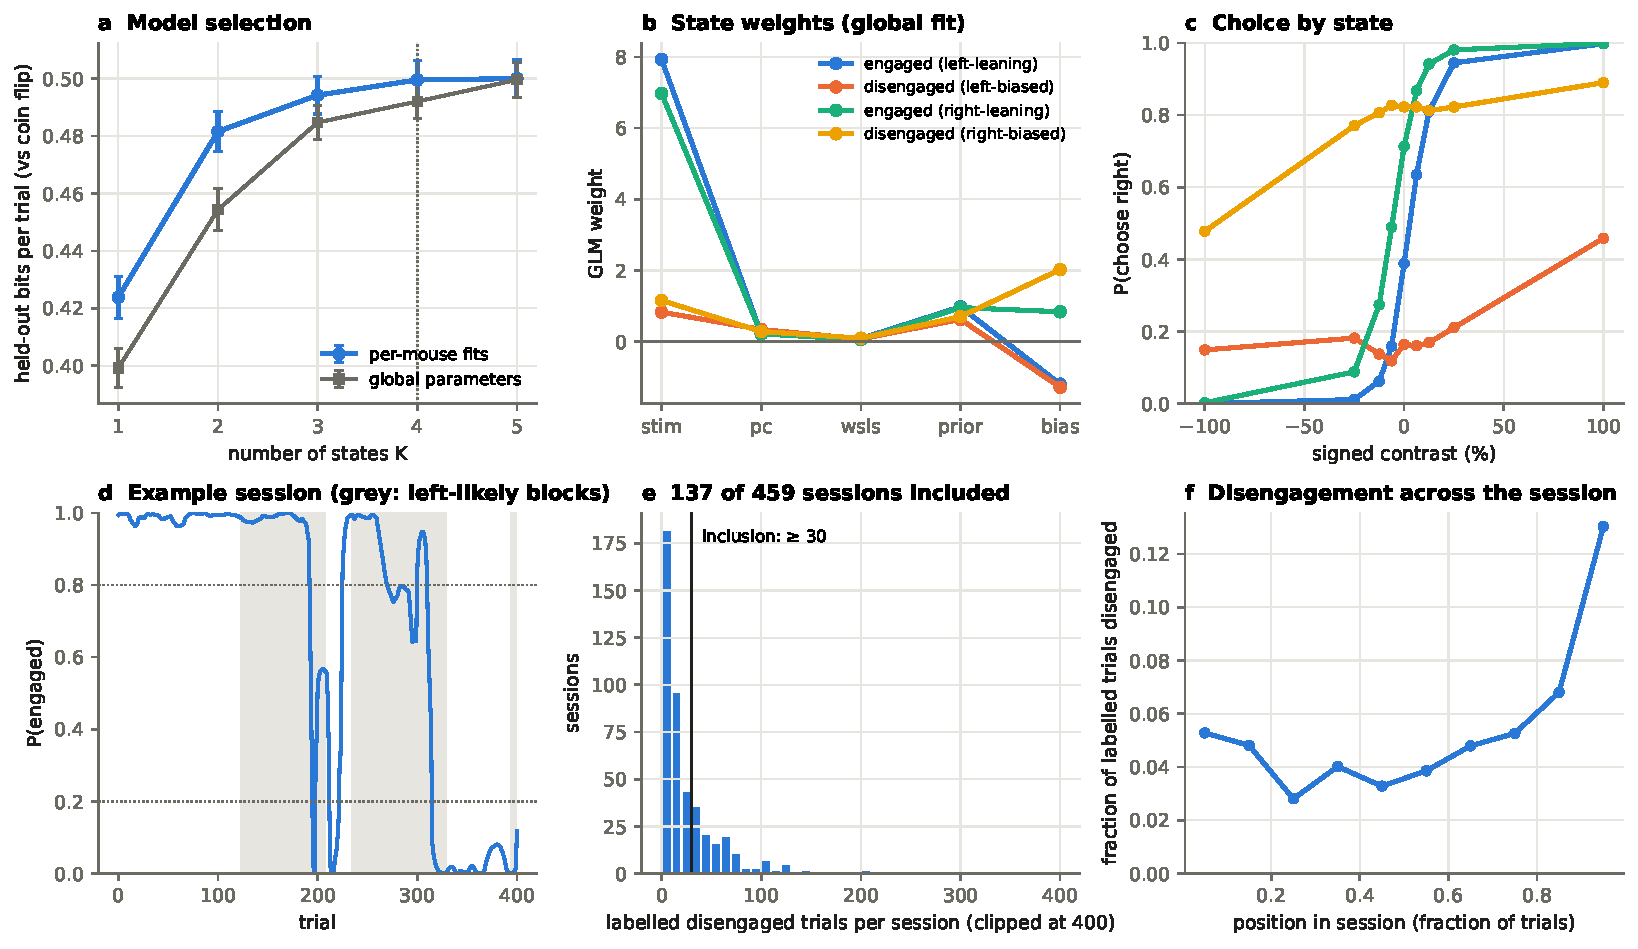
\includegraphics[width=\textwidth]{../results/figures/fig1_behaviour.pdf}
\caption{\textbf{Engagement states in Brain-Wide Map mice.} \textbf{a}, Held-out log-likelihood (bits per trial relative to a coin flip; mean $\pm$ s.e.m.\ across 114 mice) for per-mouse fits and pooled parameters; dotted line, selected $K$. \textbf{b}, GLM weights of the four states in the pooled fit. \textbf{c}, Fraction of rightward choices against signed contrast for trials assigned to each state (recording sessions). \textbf{d}, Posterior probability of the engaged states in an example session; dotted lines, labelling thresholds; grey, left-likely blocks. \textbf{e}, Labelled disengaged trials per recording session; line, inclusion threshold. \textbf{f}, Fraction of labelled trials that are disengaged, by position in the session.}
\label{fig:behaviour}
\end{figure}

\paragraph{Engagement states in the Steinmetz et al.\ data.} \todo{Filled below from the Steinmetz behaviour fit.}

\subsection{Pre-stimulus decoding of engagement across regions (H1)}
\todo{Number of sessions/mice/regions analysed; regions surviving FDR in Model B; effect sizes with CIs; brain map (Figure 3).}

\subsection{Contribution of movement, prior and time in session}
\todo{Model A vs Model B; fraction of effect retained (Figure 4).}

\subsection{Anatomical pattern (H2)}
\todo{Mixed-model contrast group H vs S.}

\subsection{Replication in Steinmetz et al.\ 2019 (H3)}
\todo{Steinmetz GLM-HMM; shared regions; Spearman $\rho$ with CI and permutation $p$ (Figure 5).}

\subsection{Robustness and exploratory analyses}
\todo{Pre-specified robustness checks; E1 (prior map), E2 (switch-aligned dynamics).}

% =====================================================================
\section{Discussion}
\todo{Draft after results.}

\section*{AI-use statement}
[AI-USE STATEMENT --- TBD]

\section*{Acknowledgements}
We thank the International Brain Laboratory and Steinmetz et al.\ for making their data openly available. \todo{Funding.}

\bibliographystyle{unsrtnat}
\bibliography{refs}
\end{document}
